\synctex=1

\documentclass{article}
\usepackage[utf8]{inputenc}

\usepackage{tikz}
\usetikzlibrary{positioning}

\begin{document}


% ---------

\begin{figure}[p]
\centering
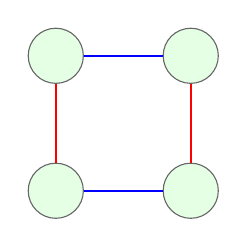
\begin{tikzpicture}[
% node style 
circ/.style={circle, draw=black!60, fill=green!10, minimum size=7mm}
],

% nodes
\node[circ] (gen_bl) {};
\node[circ] (gen_tl) [above=of gen_bl] {};
\node[circ] (gen_br) [right=of gen_bl] {};
\node[circ] (gen_tr) [above=of gen_br, right=of gen_tl] {};

% \node[circ] (gen_bl);
% \node[circ] (gen_tl) [above=of gen_bl]; % {2} label
% \node[circ] (gen_tr) [above=of gen_br, right=of gen_tl];
% \node[circ] (gen_br) [right=of gen_bl];

% draw lines between nodes
\draw[-][red, thick] (gen_tl.south) -- (gen_bl.north);
\draw[-][blue, thick] (gen_tl.east) -- (gen_tr.west);
\draw[-][blue, thick] (gen_bl.east) -- (gen_br.west);
\draw[-][red, thick] (gen_tr.south) -- (gen_br.north);

\end{tikzpicture}
\caption{Cayley diagram of the Klein 4-group}
\end{figure}

% ---------

\begin{figure}[p]
\centering
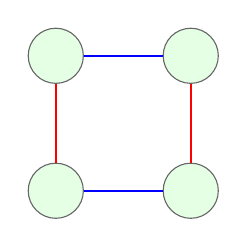
\begin{tikzpicture}[
% node style 
circ/.style={circle, draw=black!60, fill=green!10, minimum size=7mm}
],

% nodes
\node[circ] (gen_bl) {};
\node[circ] (gen_tl) [above=of gen_bl] {};
\node[circ] (gen_br) [right=of gen_bl] {};
\node[circ] (gen_tr) [above=of gen_br, right=of gen_tl] {};

% \node[circ] (gen_bl);
% \node[circ] (gen_tl) [above=of gen_bl]; % {2} label
% \node[circ] (gen_tr) [above=of gen_br, right=of gen_tl];
% \node[circ] (gen_br) [right=of gen_bl];

% draw lines between nodes
\draw[-][red, thick] (gen_tl.south) -- (gen_bl.north);
\draw[-][blue, thick] (gen_tl.east) -- (gen_tr.west);
\draw[-][blue, thick] (gen_bl.east) -- (gen_br.west);
\draw[-][red, thick] (gen_tr.south) -- (gen_br.north);

\end{tikzpicture}
\caption{Instantiation of the Klein 4-group}
\end{figure}

% ---------

\begin{figure}[p]
\centering
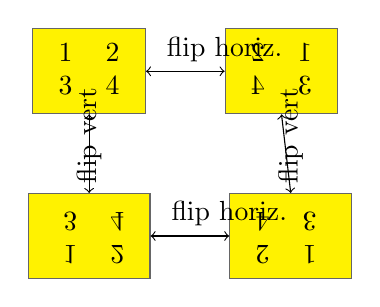
\begin{tikzpicture}[
% node style 
rect/.style={rectangle, draw=black!60, fill=yellow, minimum size=7mm}
],

% nodes
\node[rect] (gen_bl) {
  \reflectbox{\rotatebox[origin=c]{180}{
  \begin{tabular}{ l c }
  1 & 2 \\
  3 & 4 \\
  \end{tabular}}}
};
\node[rect] (gen_tl) [above=of gen_bl] {
  \begin{tabular}{ l c }
  1 & 2 \\
  3 & 4 \\
  \end{tabular}
};
\node[rect] (gen_br) [right=of gen_bl] {
  \rotatebox[origin=c]{180}{
  \begin{tabular}{ l c }
  1 & 2 \\
  3 & 4 \\
  \end{tabular}}
};
\node[rect] (gen_tr) [above=of gen_br, right=of gen_tl] {
  \reflectbox{\begin{tabular}{ l c }
  1 & 2 \\
  3 & 4 \\
  \end{tabular}}
};

% draw lines between nodes
% hack to label arrows
\draw[<->] (gen_tl.south) -- (gen_bl.north) node [above] {\rotatebox[origin=c]{90}{flip vert}};
\draw[<->] (gen_tl.east) -- (gen_tr.west) node [above] {flip horiz.};
\draw[<->] (gen_bl.east) -- (gen_br.west) node [above] {flip horiz.};
\draw[<->] (gen_tr.south) -- (gen_br.north) node [above] {\rotatebox[origin=c]{90}{flip vert}};

\end{tikzpicture}
\caption{Full map of the configuration of the rectangle puzzle}
\end{figure}

% ---------

\end{document}

%%% Local Variables:
%%% mode: latex
%%% TeX-master: t
%%% End:
